\documentclass[conference]{IEEEtran}
\IEEEoverridecommandlockouts
\usepackage{cite}
\usepackage{amsmath,amssymb,amsfonts}
\usepackage{graphicx}
\usepackage{textcomp}
\usepackage{xcolor}
\usepackage{algorithm}
\usepackage{algpseudocode}
\usepackage{booktabs}
\usepackage{subcaption}
\usepackage{tabularx}
\usepackage{url}

\def\BibTeX{{\rm B\kern-.05em{\sc i\kern-.025em b}\kern-.08em
    T\kern-.1667em\lower.7ex\hbox{E}\kern-.125emX}}
\begin{document}

\title{Auto-PET: PET Analysis framework for Urban Transit Video with Camera-Specific Cyclist and Pedestrian Detection Tuning}

\author{\IEEEauthorblockN{1\textsuperscript{st} Shayan Jalalipour}
\IEEEauthorblockA{\textit{Computer Science} \\
\textit{Portland State University}\\
Portland, Oregon \\
shayan2@pdx.edu}
\and
\IEEEauthorblockN{2\textsuperscript{nd} Banafsheh Rekabdar}
\IEEEauthorblockA{\textit{Computer Science} \\
\textit{Portland State University}\\
Portland, Oregon \\
rekabdar@pdx.edu}
}

\maketitle

\begin{abstract}
Post-Encroachment Time (PET) is useful for identifying near-miss interactions in transit conflict zones, but measuring it from fixed street-camera video still requires substantial manual review. We present an open-source RT-DETR and DeepSORT pipeline for cyclist and pedestrian detection, tracking, and PET analysis developed for bus-stop video analysis in Portland Oregon. The system addresses two practical barriers to automated PET analysis: limited labeled cyclist/pedestrian data for this camera setting, and camera-specific concept drift caused by angled mounting, object scale changes, and local geometry. Our pipeline combines semi-automated data curation, multi-stage RT-DETR fine-tuning, full-frame/top-region/perspective-warp inference, containment-aware NMS, per-class tracking, and a two-phase configuration search that tunes inference and tracker parameters without retraining the detection model. On a labeled Portland camera clip, Auto-Tuned configuration improves mAP from 0.585 to 0.767 and cyclist recall from 44.6\% to 80.4\% over the manual configuration while using the same checkpoint.\footnote{Code available at \url{https://github.com/shayan223/Cyclist-detection-using-YOLO}}
\end{abstract}

\begin{IEEEkeywords}
Post-Encroachment Time, Cyclist Detection, Pedestrian Tracking, RT-DETR, Urban Traffic Safety, Configuration Tuning
\end{IEEEkeywords}

\section{Introduction}

Post-Encroachment Time (PET) measures the time gap between one road user leaving a conflict area and another entering it. In urban transit settings, low PET values can reveal locations where pedestrians, cyclists, buses, and other vehicles interact with little temporal separation. This makes PET useful for proactive safety analysis because cities can study near misses without waiting for crash records. The bottleneck is labor: analysts must inspect long video recordings and reason about trajectories case by case.

Computer vision can reduce this cost, but street-camera PET analysis is not a solved object detection benchmark. General datasets such as COCO~\cite{lin2014microsoft}, Cityscapes~\cite{cordts2016cityscapes}, and EuroCity Persons~\cite{braun2019eurocity} are valuable, but they do not fully match fixed Portland bus-stop cameras, where overhead angled mounting makes distant cyclists small and visually different from nearby cyclists. While this use case is specific, it is but one instance of the common problem of concept drift when transferring current models and datasets to real world applications. This creates concept drift within a single frame and across camera locations. It also exposes a data availability problem: commercial transit safety systems and their datasets are not generally reproducible, while new public camera locations require local labels, warp points, thresholds, and tracker settings.

In this paper, we present a practical pipeline for automating PET analysis from City of Portland bus-stop video. The objective is not only to detect cyclists and pedestrians, but to produce stable tracked trajectories that can drive PET heatmaps to identify high risk zones and provide PET values and risk summaries of an indicated conflict zone over long periods of time. To accomplish this, we combine semi-automated data curation, RT-DETR fine-tuning, camera-aware inference, per-class DeepSORT tracking, and a PET analysis module that converts tracked actor movement into conflict-zone outputs.

This paper provides three main contributions. First, we develop a workflow for building a local cyclist/pedestrian dataset from sparse street-camera footage, reducing the amount of empty video that must be manually reviewed. Second, we build a config-driven detection and tracking pipeline that handles small distant actors through top-region and perspective-warp inference while preserving separate tracker behavior for cyclists and pedestrians. Third, we introduce an Auto-Tuned camera-specific configuration search that improves the final PET input trajectories without retraining the detector.

\section{Related Work}
\label{sec:related}

Real-time object detection has moved from single-stage convolutional detectors such as YOLO~\cite{redmon2016you} to transformer-based detectors such as DETR~\cite{carion2020end} and RT-DETR~\cite{zhao2024detrs}. RTMDet~\cite{lyu2022rtmdet} shows that careful detector design can produce strong speed/accuracy tradeoffs, while RT-DETR removes several hand-designed components and remains practical for video inference. These detectors are typically validated on broad benchmarks, but cyclist and pedestrian safety analysis from fixed transit cameras depends on local geometry, small objects, and deployment-specific thresholds. Public urban datasets help with pretraining, but they do not remove the need for local camera adaptation. We see in our own experiments that these changes in environment and data have a significant impact on model performance.

Multi-object tracking is the second requirement for PET because each actor must be followed through time. SORT~\cite{bewley2016simple} introduced a simple Kalman-filter and assignment framework, DeepSORT~\cite{wojke2017simple} added appearance-based re-identification, and ByteTrack~\cite{zhang2022bytetrack} showed the value of associating low-confidence detections rather than discarding them. We use DeepSORT because appearance cues help preserve cyclist identities when boxes shift under occlusion, perspective change, or brief detector misses. However, our experiments show that cyclists and pedestrians need different tracker parameters because they move at different speeds and have different box dynamics.

Small-object detection and perspective correction are also central in this setting. SAHI~\cite{akyon2022slicing} demonstrates that slicing can recover small distant objects, and homography-based camera work shows that inverse perspective mapping can make uncalibrated camera views more useful for traffic analysis~\cite{zhu2021monocular}. Our code supports SAHI-style tiled inference, but the reported Auto-Tuned result disables that pass; the final configuration instead relies on full-frame, top-region, and perspective-warp inference. PET has been used as a surrogate safety measure in video-based traffic analysis, including studies that model the relationship between PET and signal timing from video data~\cite{islam2022modelling}. This prior work motivates PET as a useful measure, while our work focuses on the automation layer needed to make PET analysis reproducible for fixed bus-stop camera footage.

\section{Background}
\label{sec:background}

PET is defined over a conflict area shared by two road users. If one actor leaves the conflict area at time $t_{exit}$ and another actor enters it at time $t_{entry}$, then PET is $t_{entry}-t_{exit}$ when the second actor arrives after the first has cleared the area. Lower PET values indicate smaller temporal separation between road users, which is why PET is often treated as a surrogate safety metric: it does not require an actual collision, but it can reveal interactions where the margin for error was small. In this project, the conflict area can be represented as a grid cell, a selected cell, or an interactively drawn polygon over the camera frame.

Automated PET analysis requires more than per-frame object detection. A detector can identify cyclists and pedestrians in individual frames, but PET depends on entry and exit times, which require stable actor identities across time. Tracking failures can therefore change PET measurements even when per-frame detection appears reasonable. For this reason, our pipeline treats detection, duplicate suppression, per-class tracking, and PET computation as one connected workflow rather than independent post-processing steps.

The other relevant background issue is camera-specific concept drift. In fixed transit cameras, object appearance can change dramatically inside a single frame because actors near the top of the image appear smaller, more compressed, and more affected by perspective than actors near the bottom. Between camera locations, mounting height, viewing angle, lighting, shelter placement, and sidewalk geometry also change. Homography-based perspective warp helps normalize part of this geometry by mapping a selected image quadrilateral to a rectified view, while per-class tracking allows cyclist and pedestrian motion to be handled differently after detection.

\section{Methodology}
\label{sec:method}

\begin{figure*}[t]
\centering
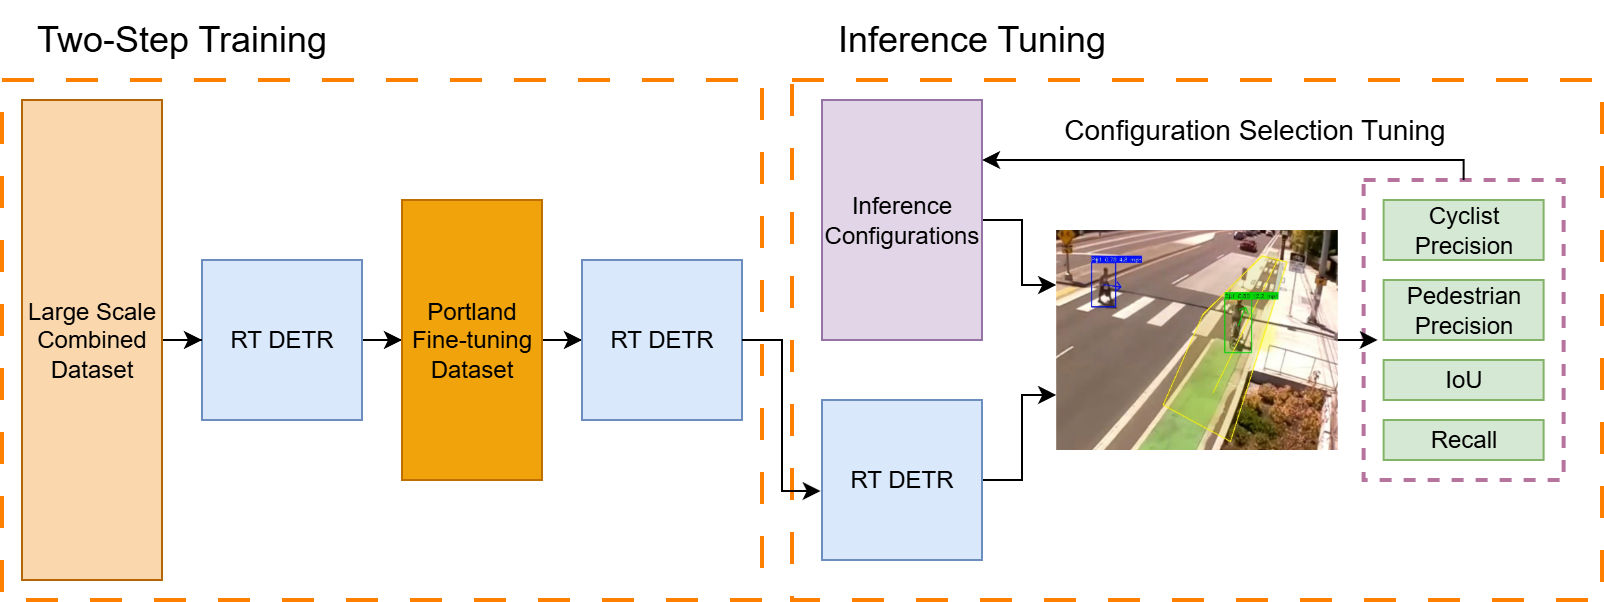
\includegraphics[width=0.95\textwidth]{pdx_cyclist_diagram}
\caption{Overview of the Portland transit-camera PET pipeline used in this work, from camera input through cyclist/pedestrian detection, per-class tracking, and conflict-zone PET computation.}
\label{fig:pdx_cyclist_diagram}
\end{figure*}

\subsection{Dataset and Data Preparation}
\label{sec:dataset}

The local Portland cyclist/pedestrian dataset is stored in YOLO format with two classes, \texttt{cyclist} and \texttt{pedestrian}. The current dataset contains 3,121 images: 2,339 train, 520 validation, and 262 test images. Frames are drawn from fixed City of Portland bus-stop cameras and split with the project splitter using a 70\%/20\%/10\% train/validation/test ratio. To reduce the amount of empty footage that must be reviewed, \texttt{movement\_window.py} uses MOG2 background subtraction, polygon ROI selection, temporal persistence filtering, and aspect-ratio, solidity, and compactness heuristics to pause on likely activity. Human labels are then saved in YOLO format with class toggling between cyclists and pedestrians.

To increase coverage before local fine-tuning, the project includes a dataset combiner that filters YOLO-format sources to cyclist/pedestrian classes, maps aliases such as \texttt{person} and \texttt{people} to \texttt{pedestrian}, maps \texttt{bike}, \texttt{bicycle}, and \texttt{biker} to \texttt{cyclist}, and removes duplicate images through MD5 hashes. A separate augmentation script can expand training data with flips, HSV jitter, translation, scale, perspective warp, large-scale jitter, top-region blur, and copy-paste of upper-frame objects, while validation and test splits are copied unchanged.

\subsection{Detection, Tracking, and PET Pipeline}

We fine-tune RT-DETR with the Ultralytics framework using the project training script defaults: 100 epochs, batch size 8, image size 640, initial learning rate 0.001, patience 10, mosaic 1.0, mixup 0.15, random erasing 0.4, horizontal flip 0.5, and RandAugment. The training curves in Fig.~\ref{fig:training_curves} show the detector learning the curated cyclist/pedestrian task: training and validation losses generally decrease, while precision, recall, and mAP improve over training. This is an important part of the story, because it indicates that the detector can fit the available labeled data. The remaining deployment challenge is not simply failed training, but the concept drift introduced by fixed street-camera geometry and camera-specific operating conditions. The trained checkpoint is fixed during all configuration-search experiments.

\begin{figure*}[t]
\centering

\includegraphics[width=0.92\textwidth]{cyclist_paper_data/RT_DETR_dataset_training_info/results.png}
\caption{RT-DETR training curves on the curated cyclist/pedestrian dataset. Losses decrease and validation precision, recall, and mAP improve, showing that the detector learns the labeled task. The later camera-specific tuning results show that strong training behavior still does not remove deployment-time concept drift from angled street-camera footage.}
\label{fig:training_curves}
\end{figure*}

At inference time, the video frame is downscaled to 960$\times$540 for the final Auto-Tuned configuration. The pipeline runs a full-frame detector pass, a top-region pass over the upper 54\% of the frame, and a warp pass using four configured homography points mapped to a 960$\times$480 rectified view. Detections from these passes are merged, clipped to frame bounds, filtered by class-specific confidence floors, and passed through hard NMS with containment cleanup followed by optional Gaussian Soft-NMS. The final Auto-Tuned NMS settings are hard IoU 0.21, containment fraction 0.57, Soft-NMS IoU 0.31, and $\sigma=0.20$. Table~\ref{tab:config_components} summarizes the configurable inference and tracking components used by the final camera-specific YAML.

Tracking uses one DeepSORT instance per class. The Auto-Tuned cyclist tracker uses \texttt{max\_age}=7, \texttt{n\_init}=1, \texttt{max\_iou\_distance}=0.84, \texttt{nms\_max\_overlap}=0.15, and \texttt{max\_cosine\_distance}=0.80. The pedestrian tracker uses \texttt{max\_age}=19, \texttt{n\_init}=3, \texttt{max\_iou\_distance}=0.40, \texttt{nms\_max\_overlap}=0.15, and \texttt{max\_cosine\_distance}=0.57. This split reflects the observation that cyclists need quick confirmation and permissive association, while pedestrians benefit from tighter matching. The SAHI option remains part of the configuration interface, but it is disabled in the reported Auto-Tuned setting because the search found better performance from the full-frame, top-region, and perspective-warp combination.

\begin{table*}[t]
\centering
\small
\caption{Inference and tracking components exposed in the final Auto-Tuned configuration. The detector checkpoint is fixed; these options change how video frames are processed, post-processed, and tracked for PET analysis.}
\label{tab:config_components}
\begin{tabularx}{\textwidth}{p{0.19\textwidth}p{0.20\textwidth}X}
\toprule
\textbf{Component} & \textbf{Final setting} & \textbf{Purpose in the pipeline} \\
\midrule
RT-DETR checkpoint & \texttt{pdx\_finetuned\_rtdetr.pt} & Fixed detector trained on the curated cyclist/pedestrian dataset. It is not changed during configuration search, so differences between configurations come from inference and tracking choices rather than retraining. \\
Frame downscaling & 960$\times$540 & Resizes each video frame before inference to reduce compute and make the camera-specific pass geometry consistent. \\
Full-frame pass & Enabled & Runs RT-DETR over the complete frame and provides the baseline set of cyclist and pedestrian detections. \\
Top-region pass & Enabled, upper 54\% & Runs a second detector pass on the upper portion of the frame, where distant actors are smaller and otherwise more likely to be missed. \\
SAHI/tiled pass & Available, disabled & Slices the image into overlapping tiles to enlarge small objects relative to the detector input. It is supported by the pipeline but was not selected by the final Auto-Tuned configuration. \\
Perspective-warp pass & Enabled, 4-point homography to 960$\times$480 & Rectifies a selected road-region quadrilateral, detects in the warped view, and maps boxes back to the original frame to improve detection under angled camera geometry. \\
Detector confidence and IoU & Confidence 0.50, IoU 0.85 & Sets the global detector confidence floor and internal detector NMS overlap tolerance before later class-specific filtering and duplicate cleanup. \\
Class confidence floors & Cyclist 0.57, pedestrian 0.73 & Applies different post-detection thresholds after all passes merge, allowing lower-confidence distant cyclists while keeping pedestrian false positives controlled. \\
Hard NMS and containment cleanup & IoU 0.21, containment 0.57 & Removes duplicate same-class boxes, including cases where one box is mostly contained inside a larger overlapping box. \\
Gaussian Soft-NMS & Enabled, IoU 0.31, $\sigma=0.20$ & Reduces scores of overlapping detections more gradually than hard suppression, which can help in crowded or partially overlapping actor regions. \\
DeepSORT tracking & One tracker per class, MobileNet embedder & Maintains actor identities over time using motion and appearance cues, producing stable trajectories required for PET entry and exit timing. \\
Cyclist tracker parameters & \texttt{max\_age}=7, \texttt{n\_init}=1, \texttt{max\_iou\_distance}=0.84, \texttt{max\_cosine\_distance}=0.80 & Confirms cyclist tracks quickly and permits larger frame-to-frame motion or appearance variation, reflecting faster movement and stronger perspective changes. \\
Pedestrian tracker parameters & \texttt{max\_age}=19, \texttt{n\_init}=3, \texttt{max\_iou\_distance}=0.40, \texttt{max\_cosine\_distance}=0.57 & Keeps slower pedestrian tracks alive longer but uses stricter association to avoid identity swaps among nearby pedestrians. \\
Debug / inference-only mode & Logging off, tracking on & Produces the final tracked video and prediction CSV rather than raw detector-only output. \\
\bottomrule
\end{tabularx}
\end{table*}

PET is computed from tracked actor histories. The pipeline uses the bottom-center of each tracked box as the ground-contact anchor and a small footprint rectangle, 40\% of box width by 20\% of box height, around that anchor. Conflict zones can be analyzed as a grid, a selected grid cell, or an interactively drawn polygon. For each pair of visits to a conflict region, PET is the time between the earlier actor's exit frame and the later actor's entry frame. Events are binned into 0--1.5 s, 1.5--3 s, 3--5 s, and 5+ s, then exported as CSV, heatmaps, and risk-over-time plots.

\subsection{Auto-Tuned Configuration Search}

Each camera has different lighting, scale, mounting, and conflict geometry, so a single YAML configuration does not transfer reliably. We therefore tune only inference and tracking parameters while keeping the detector checkpoint fixed. The search operates over the types of options listed in Table~\ref{tab:config_components}, including detector thresholds, pass settings, NMS behavior, and per-class tracker parameters. Algorithm~\ref{alg:tuning} summarizes the search.

\begin{algorithm}[t]
\caption{Camera-Specific Auto-Tuning}
\label{alg:tuning}
\begin{algorithmic}[1]
\State \textbf{Input:} seed YAML, detector checkpoint, labeled clip, $N=50$, $M=30$
\State Sample $N$ broad random YAMLs over confidence, IoU, top-region ratio, NMS, class thresholds, and tracker parameters
\For{each sampled YAML}
    \State Run inference on the labeled clip and evaluate at IoU 0.50
    \State Score trial by AP, with a penalty when mean matched IoU $<0.65$
\EndFor
\State Select top-$K$ seeds from the leaderboard
\State Allocate $M$ refinement trials across seeds, weighted by score
\State Draw Gaussian perturbations around each seed and evaluate them
\State \textbf{Output:} best camera-specific YAML and leaderboard
\end{algorithmic}
\end{algorithm}

\section{Experimental Results and Discussion}
\label{sec:experiments}

\subsection{Experimental Setup and Metrics}

We evaluate on the Camera~1 Trim~5 Portland clip using a ground-truth CSV with 544 labeled frame rows. Three configurations are compared with the same detector checkpoint: Bare bones detector-only inference, Manual Trim~5, and Auto-Tuned. Evaluation uses IoU threshold 0.50. We report mAP, class AP, final precision/recall, matched boxes, and matched-box IoU statistics. The Auto-Tuned run used seed 42, 50 exploration trials, and 30 refinement trials around the top search seeds.

Intersection over Union (IoU) measures the overlap between a predicted box and a ground-truth box divided by their union. A prediction is counted as matched when it has the correct class and IoU at least 0.50 with an unmatched ground-truth box. Precision measures how many predicted boxes are correct, while recall measures how many ground-truth boxes are recovered. Average precision (AP) summarizes the precision-recall curve for one class, and mAP averages AP across the evaluated classes. Matched boxes report the number of true-positive detections and are useful here because cyclist recall is one of the main bottlenecks for PET trajectory quality.

\begin{table}[htbp]
\centering
\caption{Detection performance on the labeled Portland camera clip at IoU=0.50.}
\label{tab:main_results}
\begin{tabular}{lcccc}
\toprule
\textbf{Configuration} & \textbf{mAP} & \textbf{Cyclist AP} & \textbf{Cyclist Rec.} & \textbf{Matched} \\
\midrule
Bare bones & 0.542 & 0.364 & 0.370 & 317 \\
Manual Trim~5 & 0.585 & 0.455 & 0.446 & 356 \\
Auto-Tuned & \textbf{0.767} & \textbf{0.818} & \textbf{0.804} & \textbf{481} \\
\bottomrule
\end{tabular}
\end{table}

Table~\ref{tab:main_results} shows that the manually configured multi-pass pipeline improves modestly over bare-bones inference, but the Auto-Tuned configuration produces the main gain. mAP increases from 0.585 to 0.767, a 31.1\% relative improvement over the manual configuration, and cyclist recall rises from 44.6\% to 80.4\%. Because the detector checkpoint is unchanged, the improvement comes from camera-specific inference, NMS, and tracker configuration rather than additional model training. Fig.~\ref{fig:iou_comparison} adds the matched-box IoU distribution, which checks that the higher match count does not come only from weaker localization.

\begin{figure}[htbp]
\centering
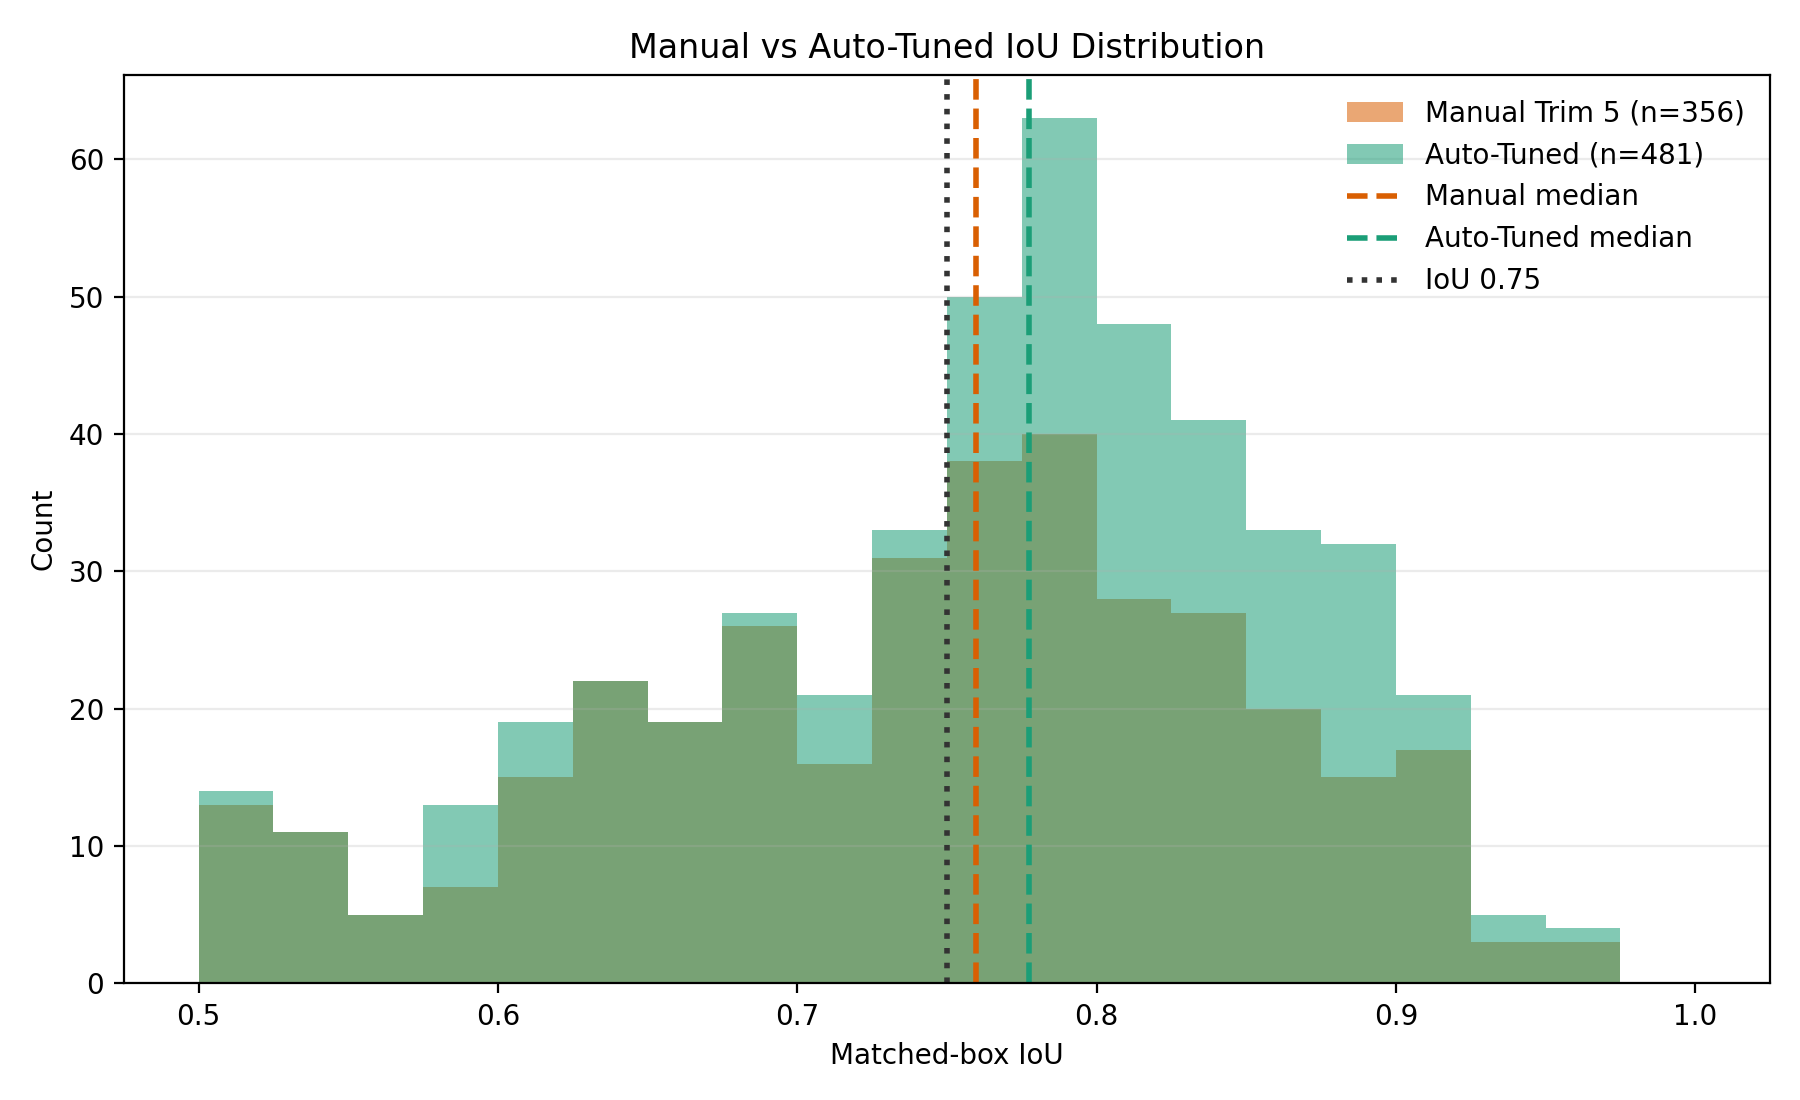
\includegraphics[width=0.98\linewidth]{cyclist_paper_data/iou_comparison.png}
\caption{Matched-box IoU distribution for Manual Trim~5 and Auto-Tuned detections. Auto-Tuned increases the matched-box count from 356 to 481 while shifting the median IoU above the manual median.}
\label{fig:iou_comparison}
\end{figure}

The tuning results reveal why camera-specific configuration matters even after successful training. As Table~\ref{tab:config_components} shows, the best configuration lowers the global confidence floor to 0.50 and the cyclist class floor to 0.57, allowing more distant cyclists to survive until tracker association and NMS. It also uses a high detector IoU setting, tight containment-aware hard NMS, a perspective-warp pass, and a permissive cyclist appearance threshold. These choices are not obvious by inspection because changing one threshold or pass can either recover small cyclists or create duplicate tracks. The two-phase search provides a reproducible way to find a workable balance between a detector that has learned the class appearance and a camera view that still shifts the apparent scale, shape, and confidence of the same actor classes.

\begin{figure}[htbp]
\centering
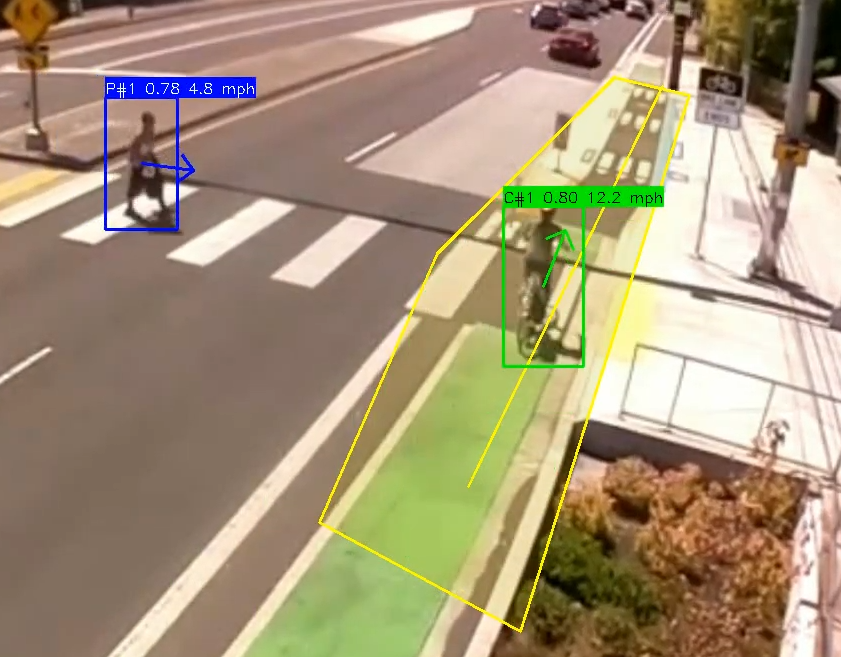
\includegraphics[width=0.92\linewidth]{cyclist_paper_data/crosswalk_direction.PNG}
\caption{Qualitative detection and tracking sample from the Portland bus-stop camera. The image shows detected pedestrian and cyclist actors, estimated direction, and the conflict area used for PET analysis.}
\label{fig:detection_sample}
\end{figure}

The pipeline also produces PET artifacts for analyst review. PET heatmaps identify conflict-zone locations where low temporal separation clusters, as shown in Fig.~\ref{fig:pet_heatmap}, and risk plots summarize low-PET events over time.

\begin{figure}[htbp]
\centering
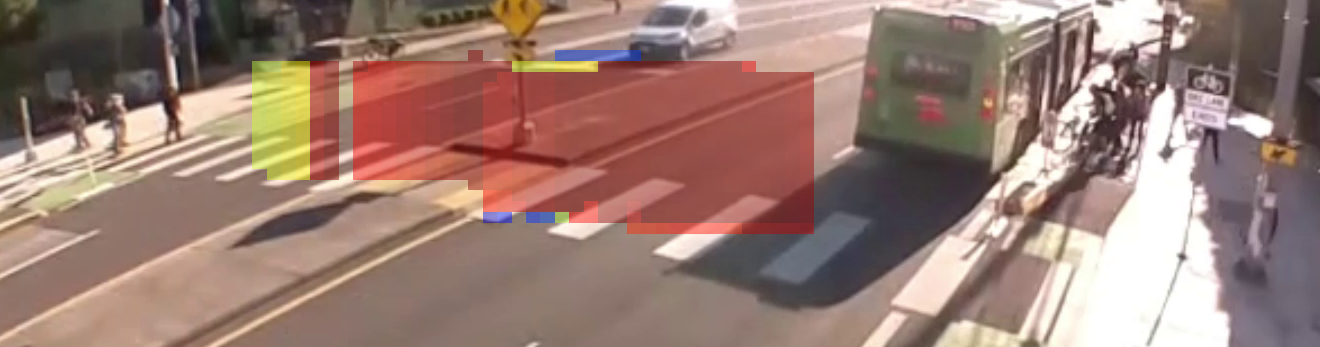
\includegraphics[width=0.76\linewidth]{cyclist_paper_data/heat_map_PET.PNG}
\caption{PET heatmap overlay for the bus-stop camera. The image is rotated to fit the column while preserving the camera-frame overlay used to identify where low temporal separation clusters.}
\label{fig:pet_heatmap}
\end{figure}

Current limitations are important. The quantitative experiment is camera-specific, the same labeled clip drives tuning and evaluation, and PET quality depends on detector/tracker stability. Future work should evaluate on additional cameras, reserve separate tuning and test clips, add nighttime footage, and compare DeepSORT with ByteTrack-style association.

\section{Conclusion}
\label{sec:conclusion}

We presented an open-source pipeline for automating PET analysis from fixed urban transit video. The system combines semi-automated data curation, RT-DETR fine-tuning, camera-aware inference, per-class DeepSORT tracking, PET heatmaps, and a two-phase Auto-Tuned configuration search. On a labeled Portland bus-stop clip, Auto-Tuned configuration improved mAP from 0.585 to 0.767 and cyclist recall from 44.6\% to 80.4\% without retraining the detector, showing that camera-specific configuration is a major lever for concept-drifted street-camera analysis. The next step is broader validation across more locations and conditions so PET automation can support scalable transit safety review.


\section{Generative AI Declaration}
Generative AI models have been used to edit and draft portions of this paper along side manual writing, rewriting, and editing. Generative AI tools were used to assist the implementation of various experiment components, but methodologies, experiment choice, and design, were created manually. All data, figures, plots, and images were created programatically with real data, and not altered or created by generative AI models.


\bibliographystyle{IEEEtran}
\bibliography{refs}

\end{document}
